\documentclass[conference]{IEEEtran}
\IEEEoverridecommandlockouts
% The preceding line is only needed to identify funding in the first footnote. If that is unneeded, please comment it out.
\usepackage{cite}
\usepackage{amsmath,amssymb,amsfonts}
\usepackage{algorithmic}
\usepackage{graphicx}
\usepackage{textcomp}
\usepackage{xcolor}
\usepackage{pgf-pie}
\usepackage{url}
\def\BibTeX{{\rm B\kern-.05em{\sc i\kern-.025em b}\kern-.08em
T\kern-.1667em\lower.7ex\hbox{E}\kern-.125emX}}

\begin{document}

    \title{Deepfake Detection\\
    }
    
    \author{
        \IEEEauthorblockN{Aadarsh Ponnuru}
        \IEEEauthorblockA{
            \textit{Department of Computer Science} \\
            \textit{National Institute of Technology Calicut}\\
        }
        
        \and
    
        \IEEEauthorblockN{Venkata Sai Vedurupaka}
        \IEEEauthorblockA{
            \textit{Department of Computer Science} \\
            \textit{National Institute of Technology Calicut}\\
        }
        
        \and
        
        \IEEEauthorblockN{Lokesh Gupta Kusumanchi}
        \IEEEauthorblockA{
            \textit{Department of Computer Science} \\
            \textit{National Institute of Technology Calicut}\\
        }
        
        \and
        
        \IEEEauthorblockN{ Lijiya A (Guide) }
        \IEEEauthorblockA{
            \textit{Associate Professor} \\
            \textit{National Institute of Technology Calicut}\\
        }
    }
    
    \maketitle
    
    \begin{abstract}
        Deepfakes are high-quality manipulated realistic videos or pictures. Though the technology has been used in legitimate applications such as for entertainment and education, etc., deep fakes have been utilized to blackmail individuals, plan terrorist attacks, disseminate incorrect facts, defame individuals as well and foment political turmoil. So there is a need for reliable methods to detect deep fakes. \\
    
        It was easier for humans to identify deepfake videos during the nascent stage of this technology owing to pixel collapse phenomena that generated visible artifacts in skin tone and the general face structure. However, with the technology’s advancement, DeepFakes have evolved to be highly indistinguishable from natural images. This project deals with the problem of detecting deepfakes.
    
    \end{abstract}
    
    % SECTIONS
    
    %% Introduction %%
    \section{Introduction}
    
        The term "Deepfake" is a blend of "Deep Learning (DL)" and "Fake", referring to highly realistic video or image content created using deep learning techniques. It first emerged in late 2017 when an anonymous Reddit user utilized deep learning to swap faces in pornographic videos, resulting in convincingly fake but realistic-looking videos. Deepfakes are produced by combining two neural networks: generative and discriminative networks, often using the FaceSwap technique. The generative network creates fake images through an encoder-decoder system, while the discriminative network assesses the authenticity of these images. This process is known as a Generative Adversarial Network (GAN), introduced by Ian Goodfellow [1]. \\
    console.
    
        Over the years, deepfakes have raised serious societal concerns due to their potential for misuse. Early deepfake videos were relatively easy to spot, with noticeable flaws such as skin tone inconsistencies, facial distortions, or visual irregularities. However, as technology has advanced, modern deepfakes have become nearly indistinguishable from real photos and videos, making it increasingly difficult to detect them with the naked eye.
    
    %% MOTIVATION %%
    \section{Motivation}
    
        The rapid advancement of artificial intelligence has revolutionized the way we create and interact with digital media, but it has also introduced significant challenges. Among these, deepfake technology stands out as a powerful yet dangerous tool that allows for the creation of highly convincing fake videos, images, and audio. This poses a serious threat not only to personal privacy but to the very fabric of trust in media and communication. The ability to fabricate false realities or manipulate content for malicious purposes—such as spreading disinformation, impersonating individuals, or causing reputational harm—underscores the urgency of addressing this issue. As deepfakes become more difficult to detect, the need for reliable detection systems has never been more critical [2]. Protecting the integrity of digital media is essential to ensuring truth and transparency in an increasingly interconnected world. 

    %% PROBLEM DEFINITION %%
    \section{Problem Definition}
    
    The objective is to design and develop a system capable of detecting deepfake videos by leveraging biological features for enhanced accuracy and reliability.

    %% LITERATURE SURVEY %%
    \section{Literature Survey}
    
        As part of our discussion, we begin by identifying the commonly used Deepfake detection techniques found in the literature. While Deepfakes typically involve the manipulation of images or videos using deep learning (DL) techniques, there are also other methods that, when combined with DL, contribute to the creation of deepfakes. In the following sections, we categorize various research efforts based on the techniques applied and provide detailed descriptions of each approach.
        
            \subsection{Machine Learning Methods}
            
            Machine learning (ML) is integral to Deepfake detection, leveraging various algorithms to analyze and identify manipulated content. Traditional ML approaches, such as Decision Trees, Random Forests, and Extremely Randomized Trees, have been effective in classifying Deepfakes based on extracted features. These methods work well in detecting patterns of manipulation but often achieve better performance when combined with more advanced techniques. \\
            
            GAN-based methods are increasingly used, not only for creating Deepfakes but also for detecting them by identifying inconsistencies that occur during the generation process. Feature-based techniques [3] focus on specific facial regions, such as the eyes or mouth, to catch abnormalities, while biological sign consistency checks for irregularities in natural signals like lip-syncing and heartbeat rhythms, offering another layer of detection. Other notable methods include 3D head pose approximation [4] for detecting unnatural movements and using Multilayer Perceptrons (MLPs) to identify visual artifacts. \\
            
            While ML methods can achieve up to 98\% accuracy under optimal conditions, their performance heavily relies on the dataset used, the features selected, and the alignment between training and testing sets. Models tend to perform well when the dataset splits are closely related, but accuracy drops significantly, sometimes to around 50\%, when tested on unrelated datasets.
            
            \subsection{Deep Learning Methods}
            
            Deep learning has revolutionized the field of deepfake detection, offering a diverse array of sophisticated techniques. These methods leverage the power of neural networks and advanced algorithms to analyze various aspects of images and videos, from facial features to subtle physiological signs. \\
            
            GAN Simulators replicate GAN-image artifacts to train classifiers, while physiological measurement techniques detect deepfakes based on subtle cues like heartbeat patterns. Inception Modules, utilizing Meso-4 and MesoInception-4 networks, focus on mean squared error for training. Convolutional Neural Networks (CNNs), both deep and shallow, have shown promising results, with deep CNNs generally outperforming their shallow counterparts. \\
            
            Feature extraction methods play a crucial role, in analyzing spatiotemporal features, common textures, and facial landmarks such as eyes, teeth, and lip movements. Data augmentation and super-resolution techniques enhance input data, improving detection accuracy. The attention mechanism allows models to focus on the most important parts of images or videos, while Capsule Networks (CN) offer efficient processing with fewer parameters than very deep networks. \\
            
            Ensemble learning combines multiple models to achieve improved accuracy, and Recurrent Neural Networks (RNNs) excel in analyzing video sequences by extracting features at both micro and macroscopic levels. Optical flow techniques [5] analyze motion between video frames, providing valuable insights into temporal inconsistencies. Autoencoder-based architectures help in reducing overfitting, while pixel-wise masking focuses on specific affected areas of the face. \\
            
            Adversarial training improves model robustness, and frequency domain analysis examines latent patterns in images that may be invisible to the naked eye. Multimodal approaches combine audio and visual analysis for a more comprehensive detection strategy. Patch-based methods focus on local image patches rather than global structures, offering a unique perspective on deepfake artifacts. \\
            
            These diverse deep learning methods collectively form a powerful toolkit for deepfake detection, each approach addressing different aspects of the challenge. By leveraging these advanced techniques, researchers and developers can create more accurate and reliable systems to combat the growing threat of deepfake technology.
            
            \subsection{Statistical Methods}
            
            Statistical methods play a crucial role in Deepfake detection by analyzing subtle discrepancies in digital media. One such method is Photo Response Non-Uniformity (PRNU), which detects unique noise patterns in images that are specific to each camera sensor. By comparing these noise patterns through normalized cross-correlation scores and applying t-tests for statistical significance, PRNU [6] helps identify manipulated content. Additionally, the Expectation-Maximization (EM) Algorithm is used to extract regional features from images, allowing for validation against various GAN architectures to detect anomalies.\\
            
            Another approach is the Statistical Framework with Hypothesis Testing, which measures the distance between the distribution of original and GAN-generated images. The method assumes that GAN-generated images deviate from the distribution of real images, and the larger this distance, the easier it is to detect Deepfakes. This framework provides a quantitative way to assess manipulations by evaluating the statistical significance of these differences.
            
            \subsection{Blockchain Methods}
            
            Blockchain methods offer a decentralized approach to Deepfake detection by ensuring content authenticity. Decentralized Verification utilizes public blockchains to track the origin of videos or images [7], linking them to trusted sources and verifying their authenticity. This method helps prevent tampering by keeping a transparent record of the content's creation.\\
            
            Another method involves IPFS-based Decentralized Storage, which integrates with the Ethereum Name Service for secure and efficient storage of media files. Additionally, LSTM Networks with Blockchain combine Long Short-Term Memory (LSTM) networks with CNNs to hash and encode media content, storing the information in a permission-based blockchain, further enhancing the security and traceability of the content.
            
    \begin{center}
        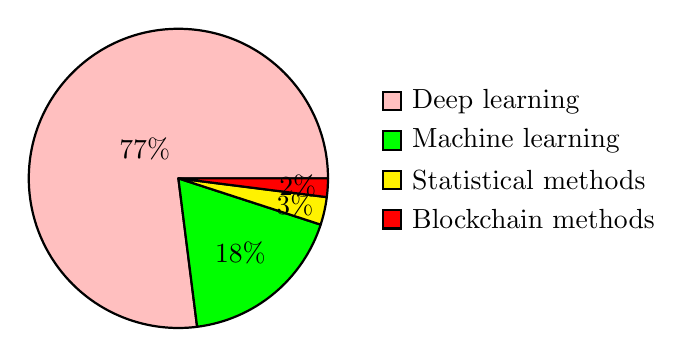
\begin{tikzpicture}
            \pie[color={pink,green,yellow,red}, 
            text=legend,
            radius=1.9]
            {77/Deep learning, 18/Machine learning, 3/Statistical methods, 2/Blockchain methods}
        \end{tikzpicture}
    \end{center}
    
    % TABLE FOR REFERENCE RESEARCH PAPERS

    %% CONCLUSION %%
    \section{Conclusion}
    
    In conclusion, while significant progress has been made in deepfake detection, the field remains dynamic and challenging. Continued research, interdisciplinary collaboration, and ethical considerations will be crucial in developing effective countermeasures against the misuse of deepfake technology. As we advance our detection capabilities, we contribute not only to the field of computer science but also to the broader goal of maintaining trust and authenticity in our increasingly digital world.

    %% REFERENCES %%
    \begin{thebibliography}{00}
    
        \bibitem{b1}  I. Goodfellow, J. P. Abadie, M. Mirza, B. Xu, D. W. Farley, S. Ozair, A. Courville, and Y. Bengio, ‘‘Generative adversarial nets,’’ in Proc. 27th Int. Conf. Neural Inf. Process. Syst. (NIPS), vol. 2. Cambridge, MA, USA: MIT Press, 2014, pp. 2672–2680
    
        \bibitem{b2} Brian Dolhansky, Joanna Bitton, Ben Pflaum, Jikuo Lu, Russ Howes, Menglin Wang, and Cristian Canton Ferrer. The deepfake detection challenge (dfdc) dataset. arXiv preprint arXiv:2006.07397, 2020.
    
        \bibitem{b3} F. Matern, C. Riess, and M. Stamminger, ‘‘Exploiting visual artifacts to expose deepfakes and face manipulations,’’ in Proc. IEEE Winter Appl. Comput. Vis. Workshops (WACVW), Waikoloa Village, HI, USA, Jan. 2019, pp. 83–92.
    
        \bibitem{b4} X. Yang, Y. Li, and S. Lyu, ‘‘Exposing deep fakes using inconsistent head poses,’’ in Proc. IEEE Int. Conf. Acoust., Speech Signal Process. (ICASSP), Brighton, U.K., May 2019, pp. 8261–8265.
    
        \bibitem{b5} I. Amerini, L. Galteri, R. Caldelli, and A. Del Bimbo, ‘‘Deepfake video detection through optical flow based CNN,’’ in Proc. IEEE/CVF Int. Conf. Comput. Vis. Workshop (ICCVW), Oct. 2019, pp. 1205–1207.
    
        \bibitem{b6} M. Koopman, A. M. Rodriguez, and Z. Geradts, ‘‘Detection of deepfake video manipulation,’’ in Proc. 20th Irish Mach. Vis. Image Process. Conf. (IMVIP), London, U.K., 2018, pp. 1–4.
    
        \bibitem{b7} H. Hasan and K. Salah, ‘‘Combating deepfake videos using blockchain and smart contracts,’’ IEEE Access, vol. 7, pp. 41596–41606, 2019.
    
    \end{thebibliography}
    
    % \vspace{12pt}
    % \color{red}
    % IEEE conference templates contain guidance text for composing and formatting conference papers. Please ensure that all template text is removed from your conference paper before submission to the conference. Failure to remove the template text from your paper may result in your paper not being published.
    
\end{document}
